\vspace{-7pt}
\section{Method}
\vspace{-5pt}
\label{sec:method}

In this section, we first formulate the problem, then present COD in four stages (see \cref{fig:main-pipeline}).
(1) We construct sample-level difficulty scaling features and apply an improved MeanShift clustering algorithm (\cref{sec:method-clustering}).
(2) We derive a performance scaling law with respect to task difficulty variance, enabling extrapolation of performance–compute relationships for clusters with similar difficulty features. Cluster-wise curves are fitted on small models to identify extrapolatable clusters (\cref{sec:fitting}).
(3) We extrapolate performance for these clusters to predict the target large model’s accuracy on the predictable subset (\cref{sec:extrapolation}).
(4) Finally, we map subset accuracy to full evaluation results (\cref{sec:mapping}).

\textbf{Problem Formulation.} Consider a language model $M_C$ trained with a compute budget of $C$ measured in FLOPs. Let $\mathcal{P}$ be a set of downstream tasks that we aim to evaluate the model on. Each sample $T \in \mathcal{P}$ is defined by a question-answer pair $(q, a_{\text{true}})$. Given a question $q$, the model $M_C$ outputs a probability distribution $p(a|q; M_C)$ over the space of all possible answers.

% \labubu{For a task instance $(q, a_{\text{true}})$ where the answer is a token sequence $a_{\text{true}} = (t_1, t_2, \ldots, t_k)$, the Next-Token-Prediction loss $L(q, a_{\text{true}}; C)$ is defined as the sum of the negative log-probabilities of the ground-truth tokens:}

% $$L(q, a_{\text{true}}; C) = -\sum_{i=1}^{k} \log p(t_i | q, t_{<i}; M_C)$$

Our goal is to predict the downstream task performance of a large language model $M_{C_{\text{target}}}$ using only evaluation results from smaller models $\{M_{C_1}, M_{C_2}, \ldots, M_{C_n}\}$ where $C_i \ll C_{\text{target}}$ for all $i$. Formally, we aim to find the prediction method $\phi$ to minimize the absolute prediction error over a group of tasks sets $\{\mathcal{P}_j\}_m$:
$$\arg\min_{\phi}\frac{1}{m}\sum_{i=1}^m\frac{1}{|\mathcal{P}_j|}\sum_{T\in \mathcal{P}_j}\vert\widehat{\text{Acc}}(C_{\text{target}}, T)-\text{Acc}(C_{\text{target}})\vert,$$
$$\widehat{\text{Acc}}(C_{\text{target}}, T) := \phi\left(\{\text{Acc}(C_i, T)\}_{i=1}^{n}, \{C_i\}_{i=1}^{n}, C_{\text{target}}\right),$$
where $\text{Acc}(C, T)$ denotes the accuracy of model $M_C$ on task $T$, and $\widehat{\text{Acc}}(C_{\text{target}}, T)$ is the predicted accuracy for the target model.


\subsection{Clustering on Difficulty}
\label{sec:method-clustering}

\camera{Although downstream tasks in the same evaluation set share similar themes, they exhibit significant differences in difficulty, resulting in distinct performance scaling patterns that make a universal fitting function inapplicable.} We propose clustering tasks by similar performance scaling behaviors to minimize intra-cluster heterogeneity maintaining a minimum cluster size.

Specifically, we train a group of language models with increasing parameter counts. These models are trained with the same ratio of training tokens to compute per token. %我们采用和预估阶段相同一组小模型来评测任务的难度特征，不会引入大模型评测结果以避免信息泄露额。
\revise{We use the same set of small models for prediction to evaluate the difficulty characteristics of the task, and will not introduce the target large model evaluation results to avoid feature leakage.}

For each task, we generate 100 samples using \texttt{top\_p}=0.7 and \texttt{temperature}=1.0 for each model, and compute the pass rate by averaging the results. This pass rate serves as an estimate of the model’s expected accuracy on the task. The resulting values are \revise{concatenated} into a difficulty vector, ordered by increasing model size. For most tasks, this difficulty vector exhibits a monotonic increase, reflecting the gradual improvement of model capability with scale.



\begin{figure*}[!t]
    \centering
    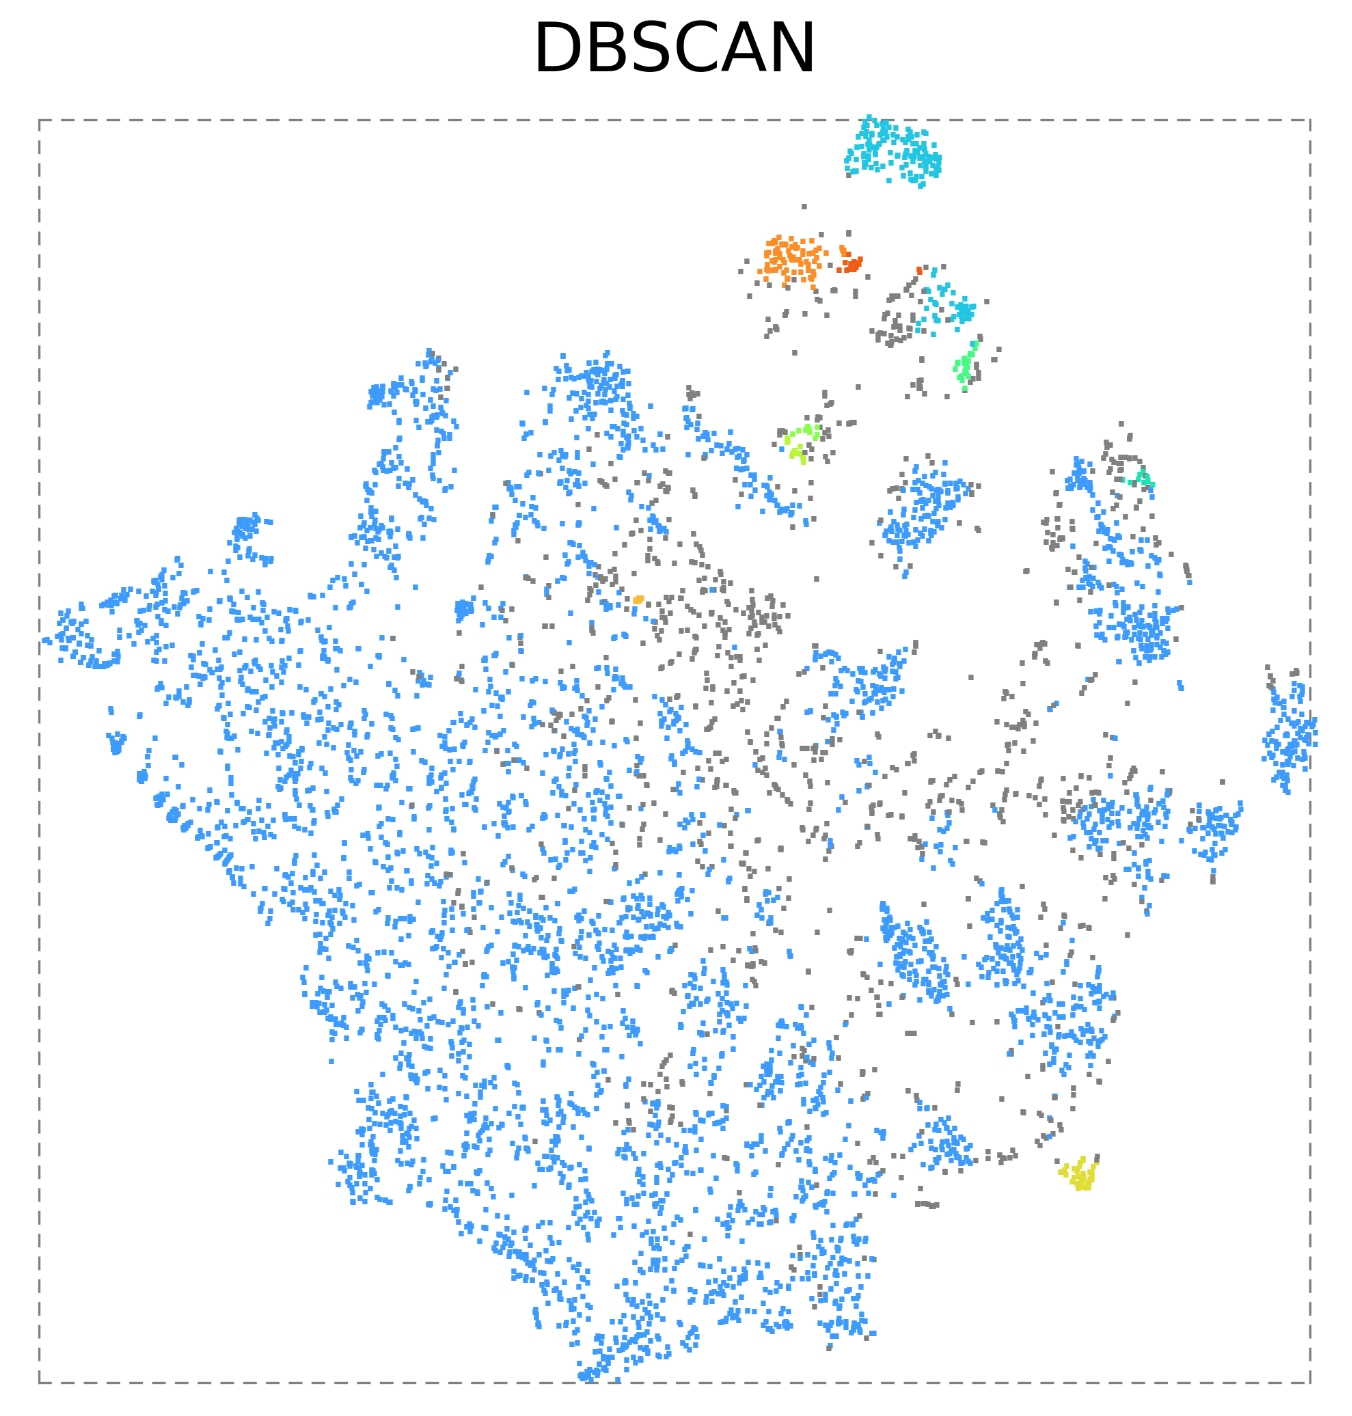
\includegraphics[width=0.28\textwidth]{figures/method/DBSCAN_BBH_v2.jpeg}
    \hspace{0.03\textwidth}  % 调整两图之间的间距
    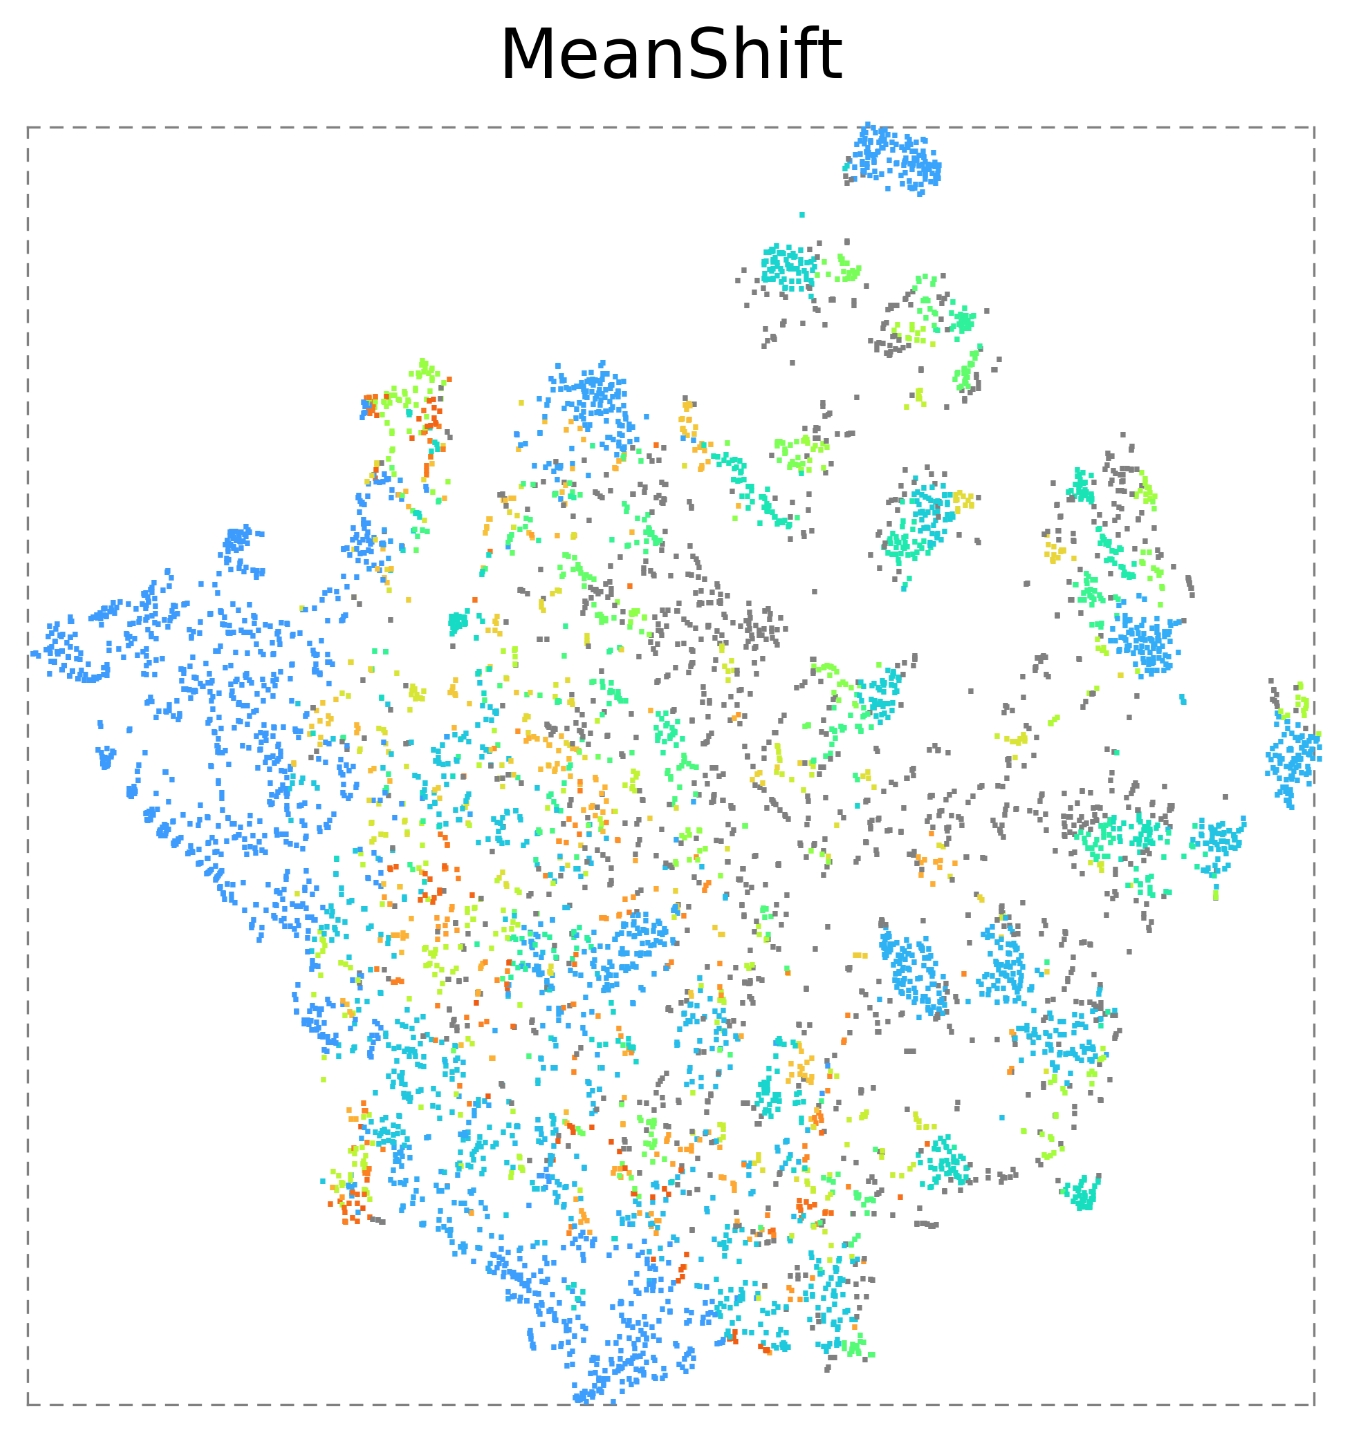
\includegraphics[width=0.28\textwidth]{figures/method/MeanShift_BBH_v2.jpeg}
    \hspace{0.03\textwidth}  % 调整两图之间的间距
    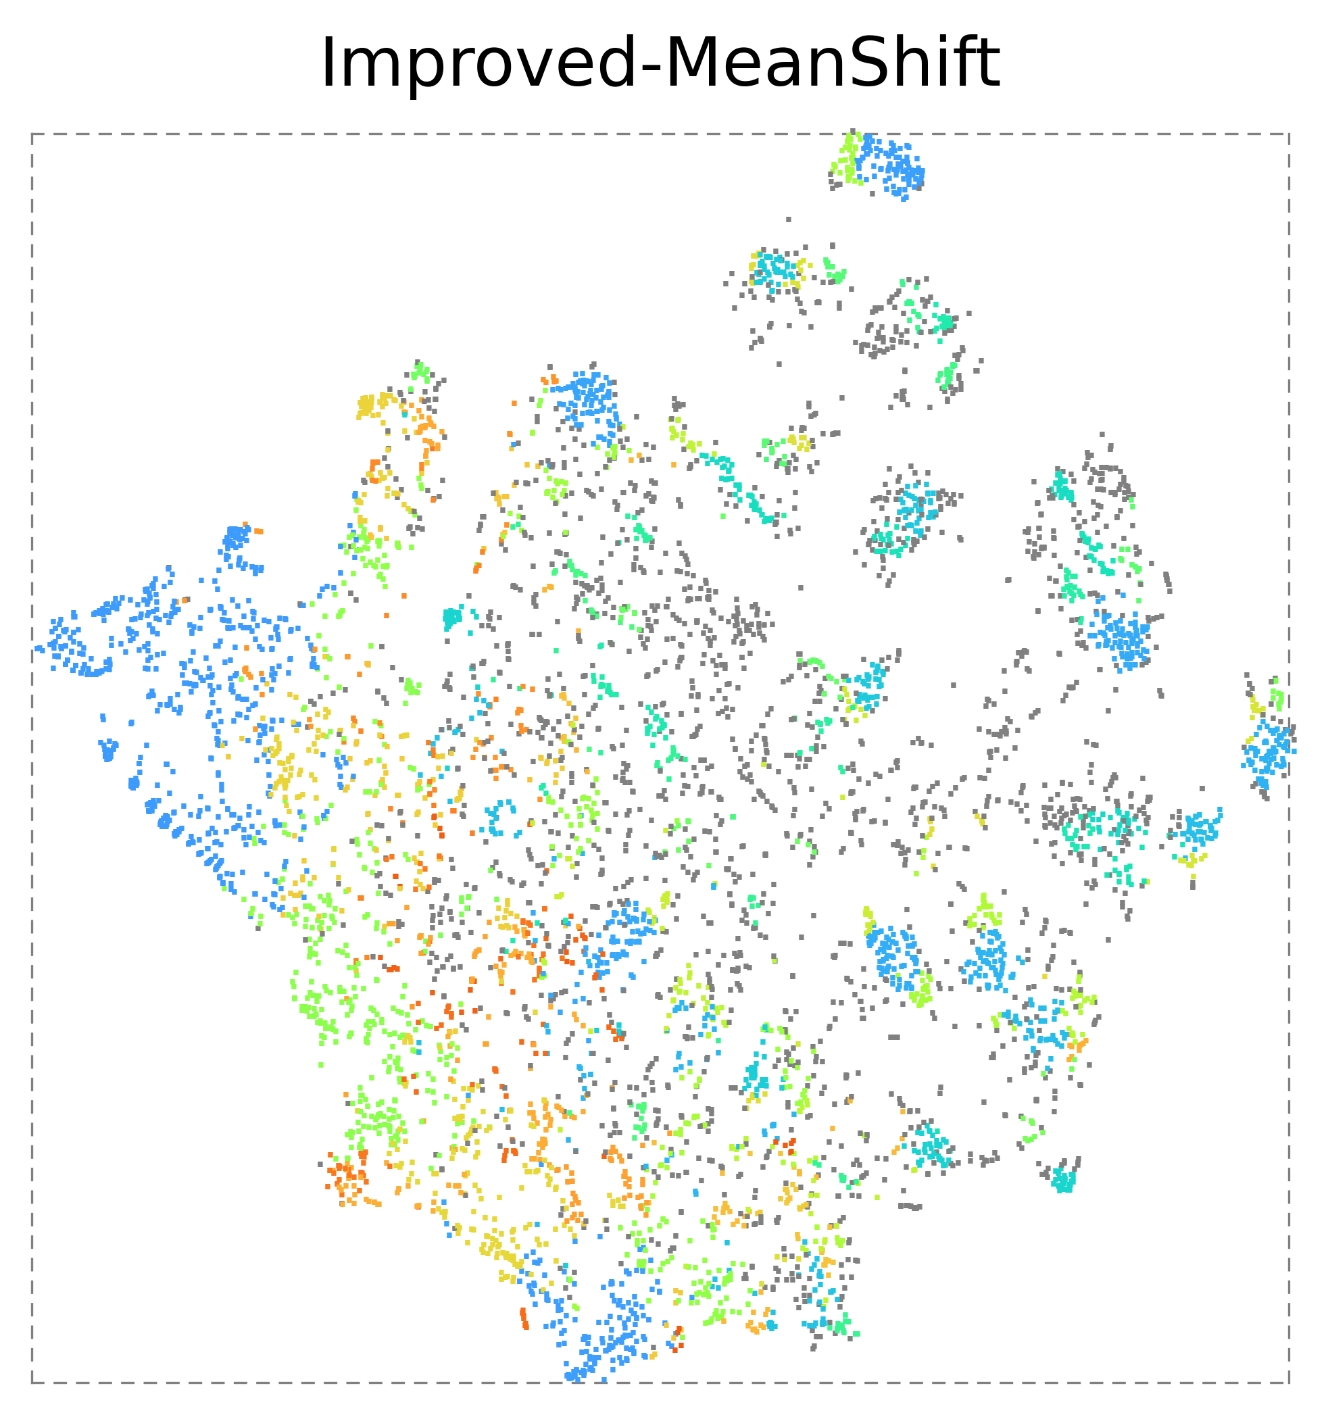
\includegraphics[width=0.28\textwidth]{figures/method/ImprovedMeanShift_BBH_v2.jpeg}
    \caption{t-SNE visualization of different clustering methods: DBSCAN(left), MeanShift(Middle), Improved-MeanShift(Right). Each point represents an evaluation sample. }
\label{fig:tsne_vis}
\vspace{-10pt}
\end{figure*}

After obtaining the difficulty feature vector for each task, we use the improved clustering algorithm that incorporates the following features:
(1) Minimizing intra-class variance to ensure similar extrapolation properties within each cluster;
(2) Automatic determination of cluster numbers, as the optimal number varies across evaluation sets and is difficult to pre-specify. 

% K-Means~\citep{macqueen1967some} requires pre-specifying cluster numbers and DBSCAN~\citep{ester1996density} may yield large intra-cluster variance, MeanShift~\citep{fukunaga1975estimation} allows constraining this variance via a radius parameter, better suiting our needs.

To further reduce intra-class variance, we propose an improved MeanShift algorithm to constrain the cluster diameter. At the same time, we maintain a minimum number of tasks in each cluster to reduce metric fluctuations.
We provide the t-SNE visualization of clustering results evaluation tasks on BBH~\citep{suzgun2023challenging} to compare the proposed method and classic clustering algorithms including DBSCAN~\citep{ester1996density} and MeanShift~\citep{fukunaga1975estimation}. Each point represents an evaluation sample, and its color denotes the cluster type. As shown in \cref{fig:tsne_vis}, our improved MeanShift effectively splits dense areas whereas DBSCAN and the original MeanShift produce connected clusters with large within-cluster distances.

We provide numerical comparison of clustering algorithms in~\cref{sec:clustering_ablation} and explain implementation details of improved MeanShift in Appendix~\ref{sec:improved},  smoothing techniques in Appendix~\ref{sec:smoothing}. 

% We also cast an ablation study on clustering methods in \cref{sec:clustering_ablation}.


\subsection{Fitting}
\label{sec:fitting}
% 得到聚类结果后，我们在每个类簇上计算评估指标，并完成独立的外推曲线拟合。
% 我们给出Scaling Law for Downstream Task Performance以及对应的理论分析, 并可以从中推导出难度特征相似的类簇上的Performance scaling预测公式。

After clustering, we compute metrics for small models within each cluster.
\camera{We then fit the accuracy-compute curves for each cluster using a theoretically derived novel performance scaling law}, focusing on clustered samples after excluding outliers. We derive the following fitting formula for the downstream task scaling law based on the training loss scaling law.


\begin{theorem}[Scaling Law for Downstream Task Performance]
\label{main:proof:task_scaling_law}
Consider a language model $M_C$ trained with compute budget $C$ and a set of downstream tasks $\mathcal{P}$. Under the following assumptions:
Assumption 1 (Power-law scaling of answer loss): the expected answer loss follows:
\begin{equation}
L_{\mathcal{P}}(C) := \mathbb{E}_{(q,a_{\text{true}}) \sim \mathcal{P}}[L(q, a_{\text{true}}; C)] = \alpha C^{-\beta} + \gamma,
\end{equation}
where $\alpha, \beta, \gamma > 0$ are task-specific constants, with $\gamma$ representing the irreducible loss.

Assumption 2 (Unique deterministic answers): Each question has a unique deterministic answer. The model receives score $1$ if and only if $M_C$ outputs $a_{\text{true}}$, and $0$ otherwise.

Assumption 3 (Accuracy decomposition): The expected accuracy decomposes as:
\begin{equation}
\mathbb{E}_{T \sim \mathcal{P}}[\mathrm{Acc}(C)] = g + (1-g) \cdot \mathbb{E}_{(q,a_{\text{true}}) \sim \mathcal{P}}[p(a_{\text{true}}|q, M_C)],
\end{equation}
where $g \in [0,1]$ is the random guessing baseline.

Then, the expected accuracy on task set $\mathcal{P}$ can be modeled as:
\begin{equation}
\mathbb{E}_{\mathcal{P}}[\mathrm{Acc}(C)] =g+(1-g)\left(\exp{(-\alpha C^{-\beta}-\gamma)} + \frac{\sigma_L^2(C)}{2\mu_L(C)} \right)+ o\left(\sigma_L^2(C)\right), 
\end{equation}
where $\mu_L(C) = \mathbb{E}_{(q,a_{\text{true}}) \sim \mathcal{P}}[L(q, a_{\text{true}}; C)]$ is the mean loss and $\sigma_L^2(C) = \mathrm{Var}_{(q,a_{\text{true}}) \sim \mathcal{P}}[L(q, a_{\text{true}}; C)]$ is the loss variance across the task set.
\end{theorem}


\begin{proof}[Proof Sketch]
By definition of the language model loss, $p(a_{\text{true}}|q, M_C) = \exp(-L(q, a_{\text{true}}; C))$. Under Assumption 1, if the answer loss follows a power law $L \sim \alpha C^{-\beta} + \gamma$, then the task passrate should approximately scale as $\exp(-\alpha C^{-\beta} - \gamma)$.

The key subtlety lies in the averaging: accuracy computes $\mathbb{E}[\exp(-L)]$ (arithmetic mean of passrates) while the loss scaling law gives us $\exp(-\mathbb{E}[L])$ (geometric mean). Using Taylor expansion:
$$\mathbb{E}[\exp(-L)] \approx \exp(-\mu_L) \ + \frac{\sigma_L^2}{2\mu_L},$$
where $\mu_L$ and $\sigma_L^2$ are the mean and variance of the loss distribution.

This approximation is accurate when tasks have similar difficulty feature ($\sigma_L^2/\mu_L^2 \ll 1$), motivating our clustering approach to reduce intra-cluster variance. Assumption 3 adds the parameter $g$ for random guessing. The complete proofs are provided in Appendix~\ref{sec:prop_proof}.
\end{proof}
\cref{main:proof:task_scaling_law} demonstrates that a metric of an evaluation set with similar difficulty features can be effectively modeled using the following formula:
\begin{equation}
y(C)=g+(1-g)*e^{-aC^{-b}-c},
\label{eq:fitting}
\end{equation}
where $a$ and $b$ jointly influence how accuracy varies with $C$, while $c$ constrains the upper bound of the fitting curve, and $g$ represents the expected random guess metric for a task cluster. 
$a$, $b$, $c$, and $g$ are trainable parameters. 
Note that these assumptions may not perfectly hold in practice, we provide additional discussions on assumption 3 in Appendix~\ref{sec:limiations}.


\subsection{Extrapolation}
\label{sec:extrapolation}

To ensure reliable extrapolation, we identify clusters exhibiting robust scaling patterns, as some clusters may show saturated or non-emergent performance on smaller models, making them unsuitable for prediction. We aim to find an extrapolation subsets that represent the full set performance, and use the subset metric as a intermediate indicator for the prediction of the full set accuracy.

A cluster is deemed \textbf{extrapolatable} if it meets two criteria: (1) its expected accuracy increases monotonically with model size, and (2) its performance converges to at least a predefined threshold~$P$ (where $P \leq 1$ accounts for practical limits like ambiguous questions or finite training coverage). 

We filter out non-extrapolatable clusters using two rules based on the parameters from \cref{eq:fitting}:
\begin{enumerate}[leftmargin=1.5em]
    \item Negligible accuracy growth, indicated by minimal $a$ or $b$ values.
    \item Poor extrapolation reliability, indicated by an excessive $c$ value.
\end{enumerate}
In practice, for extrapolatable clusters, we set $a > 1$, $b > 0.1$, and $0 \leq c < 1$. \anno{Further ablation experiments are provided in Appendix~\ref{sec:criteria}.}

The clusters satisfying these conditions form the \textit{predictable subset}. The final performance prediction for a target model on this subset is the weighted average of the extrapolated predictions from these individual clusters, with weights proportional to cluster sizes.

% \subsection{Mapping from Predictable Subset to Target Evaluation Set}
% \label{sec:mapping}
% We map predictions from the predictable subset $\mathcal{P}'$ to the complete evaluation set $\mathcal{P}$ using a \camera{smooth} function. This approach is based on the observation that extrapolatable and non-extrapolatable samples, while differing in difficulty, often share question types, suggesting a preserved relative metric ordering. The mapping function $f: \text{Acc}(\mathcal{P}') \rightarrow \text{Acc}(\mathcal{P})$ is continuous, smooth over $[0,1]$, monotonically increasing, and constrained to pass through $(0,0)$ and $(1,1)$. Empirical validation indicates a polynomial function optimally captures this relationship:
% \begin{equation}
%     f_n(x)=\alpha_{n-1}x^n+\alpha_{n-2}x^{n-1}+...+\alpha_1x^2+(1-\alpha_1-\alpha_2-...-\alpha_{n-1})x,
%     \label{eq:mapping}
% \end{equation}
% \anno{where $x$ represents the average accuracy of the predictable subset $\mathcal{P}'$, and 
% $n$ denotes the highest degree of the polynomial. In practical implementation, a quartic function is employed to fit the mapping (see Appendix~\ref{sec:interpolation_ablation} for exhaustive experimental details).} To ensure reliability, we calibrate $f$ using evaluation results from existing models as anchors. This subset-to-full mapping generally demonstrates robustness across diverse model architectures and training data, often permitting the use of external models (e.g., Qwen2-72B~\citep{yang2024qwen2}) as anchors for many tasks (see Appendix~\ref{sec:anchor} for experiments). However, for data-sensitive tasks, models with similar training distributions provide more reliable anchors, prioritizing data consistency for mapping accuracy. The final metric prediction for a target LLM with estimated training computation $C_0$ is then $p = f \circ y(C_{0})$, combining the cluster-wise extrapolation $y(C_0)$ from \cref{eq:fitting} with the mapping $f$.

\camera{\subsection{Mapping from Predictable Subset to Target Evaluation Set}
\label{sec:mapping}
We map predictions from the predictable subset $\mathcal{P}'$ to the complete evaluation set $\mathcal{P}$ using a smooth function. This mapping strategy is motivated by the observation that extrapolatable and non-extrapolatable samples, despite their difficulty differences, usually belong to the same question types, which implies a consistent relative metric ordering between the predictable subset and the full evaluation set. The mapping function $f: \text{Acc}(\mathcal{P}') \rightarrow \text{Acc}(\mathcal{P})$ is continuous, smooth over $[0,1]$, monotonically increasing, and constrained to pass through $(0,0)$ and $(1,1)$. Empirical validation indicates that a smoothing spline optimally captures this relationship. Specifically, we employ a cubic smoothing spline to model the mapping.
where $x$ represents the average accuracy of the predictable subset $\mathcal{P}'$. In practical implementation, under the premise of fixing the curve to pass through $[0,0]$ and $[1,1]$, we determine the number of piecewise cubic segments (knots) by setting a Root Mean Square Error (RMSE) fitting threshold of $0.005$. The number of segments is dynamically adjusted until the fitting RMSE meets this threshold. 
We list the implementation details and visualization of mapping in \cref{sec:interpolation_ablation}.

To ensure reliability, we calibrate $f$ using evaluation results from existing models as anchors. This subset-to-full mapping generally demonstrates robustness across diverse model architectures and training data, often permitting the use of external models (e.g., Qwen2-72B~\citep{yang2024qwen2}) as anchors for many tasks (see Appendix~\ref{sec:anchor} for experiments). The final metric prediction for a target LLM with estimated training computation $C_0$ is then $p = f \circ y(C_{0})$, combining the cluster-wise extrapolation $y(C_0)$ from \cref{eq:fitting} with the mapping $f$.}